%%%%%%%%%%%%%%%%%%%%%%%%%%%%%%%%%%%%%%%%%%%%%%%%%%%%%%%%%%%%%%%%%%%%%%%
\chapter{System Models in Different Domains}
\label{ch:systemmodels}
%%%%%%%%%%%%%%%%%%%%%%%%%%%%%%%%%%%%%%%%%%%%%%%%%%%%%%%%%%%%%%%%%%%%%%%


\section{Electrical circuits and networks}

Any electrical circuit can be modelled by a bond graph containing elements of the set $\{ 0, 1, R, C, I, Se, Sf \}$. For electrical circuits the mapping to bond graph variables is direct: voltage is effort, current is flow. The 0-junction encodes Kirchhoff's current law at a node (same voltage, currents sum to zero); the 1-junction encodes Kirchhoff's voltage law around a loop (same current, voltage drops sum to zero).

$TF$ and $GY$ are not included since they are used to represent electrical networks.

\begin{itemize}
  \item 0 Junction: Same voltage
  \item 1 Junction: Same current
\end{itemize}


\paragraph{Construction procedure.}
Constructing the overall bond graph model is much easier if a procedure can be followed that ensures success regardless of the complexity.

\begin{figure} [H]
\centering 
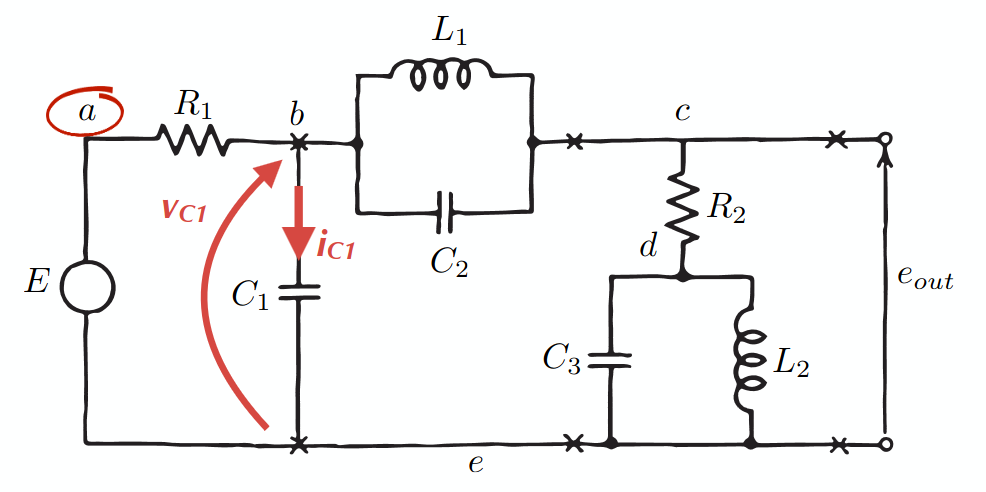
\includegraphics[scale=0.25]{figs/chapter3/3_1.png}
\caption{Example of electric circuit}
\end{figure}

\begin{enumerate}[leftmargin=2em,itemsep=2pt]
  \item \textbf{Assign a power convention}: for each circuit element choose positive current direction and positive voltage drop. Talking about power in BG, we typically ensure that, when positive, power is flowing \emph{towards} the passive 1-port element. Note that active elements are elements providing power (sources, but also energy-storing elements freeing their energy). In some situations, sources may even absorb power.
  \item \textbf{One 0-junction per node voltage}: place a 0-junction for every distinct node voltage (including what will be the ground). Every bond touching a 0-junction carries the same effort (node voltage).
  \item \textbf{One 1-junction per element}: for each circuit element (R, L, C, source), insert a 1-junction to represent the voltage difference across it. By properly directing the half-arrows on 1-junctions, the voltage drop can be established across each element. Connect the 1-junction between the two 0-junctions at its terminals. Attach the bond graph element (R, I, C, Se, Sf) to the 1-junction.
  \item \textbf{Ground = zero effort source}: choose a ground node and connect the ground 0-junction to a Sf~: 0 (zero-flow source) or Se~: 0 (zero-voltage), which in practice means deleting all bonds with zero power at that junction. Note that different bond graphs will result for a given circuit if we choose different ground nodes.7


  \begin{figure} [H]
  \centering
  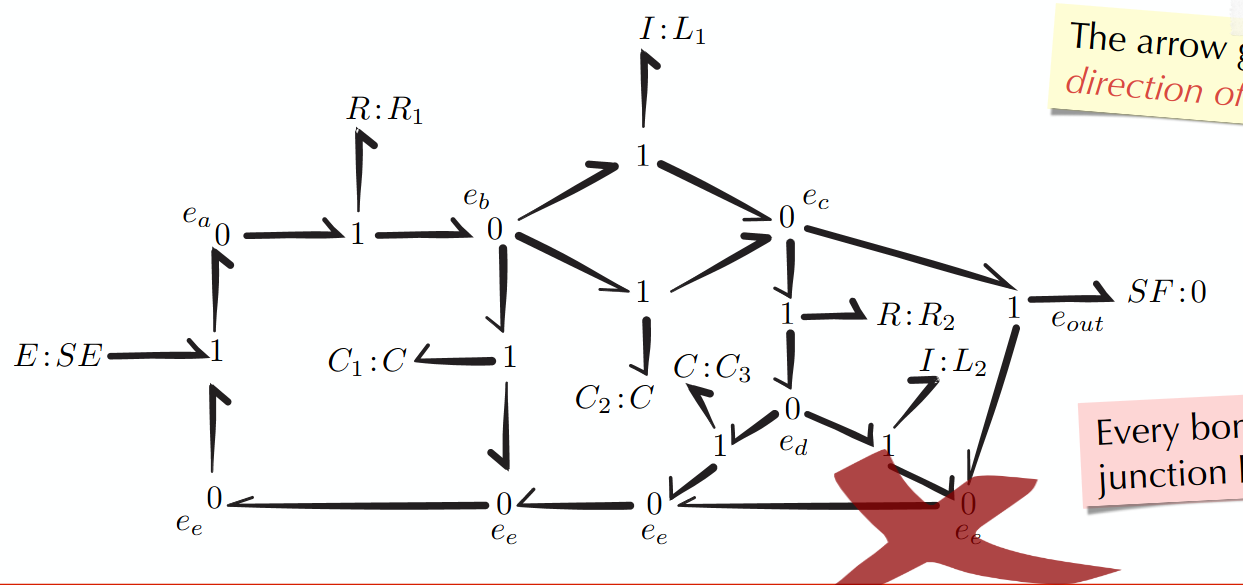
\includegraphics[scale=0.25]{figs/chapter3/3_2.png}
  \caption{Example of bond graph construction for the circuit in Fig. 3.1.}
  \end{figure}



  \item \textbf{Simplify}: apply bond graph identities to remove redundant junctions and bonds.
\end{enumerate}

\begin{figure} [H]
\centering
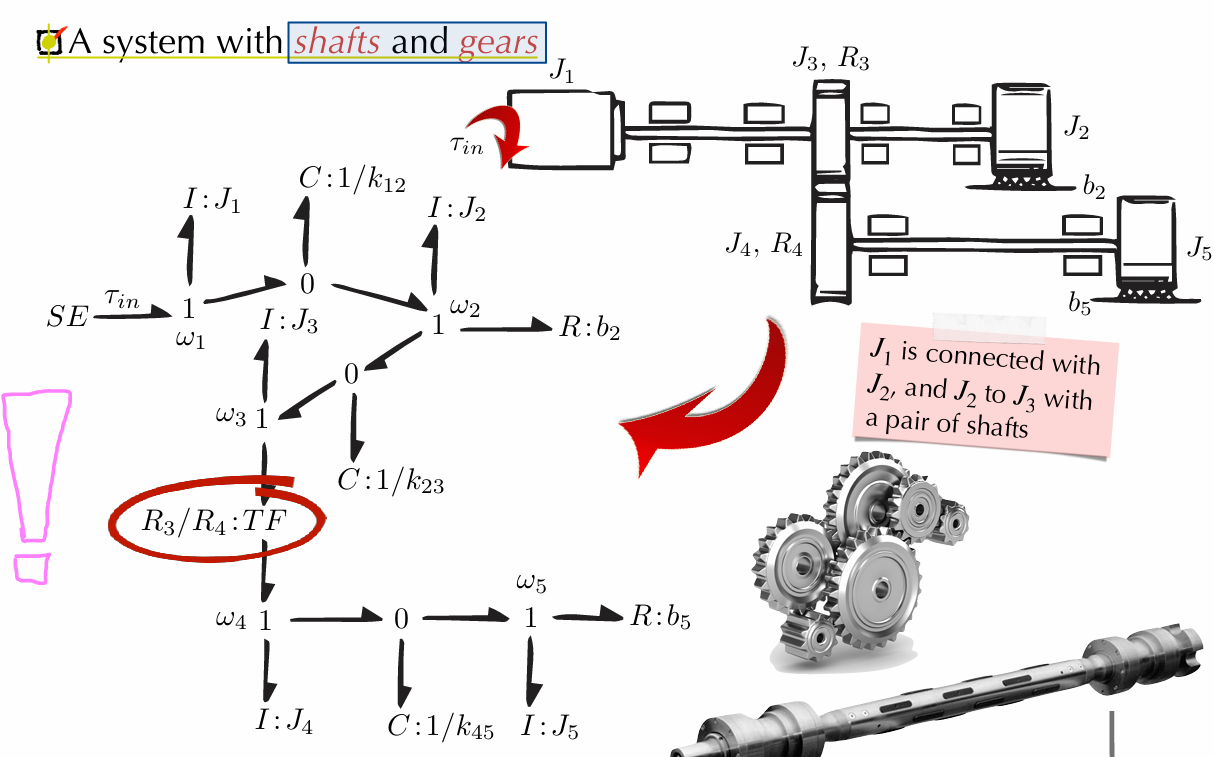
\includegraphics[scale=0.25]{figs/chapter3/3_3.png}
\caption{Example of bond graph simplification.}
\end{figure}


An electrical network is an extension of electrical circuits to include idealised transformers $TF$ and gyrators $GYG$. 



\subsubsection{Electrical Transformers}
It's used used to to step voltages up or down. 

\begin{figure} [H]
\centering
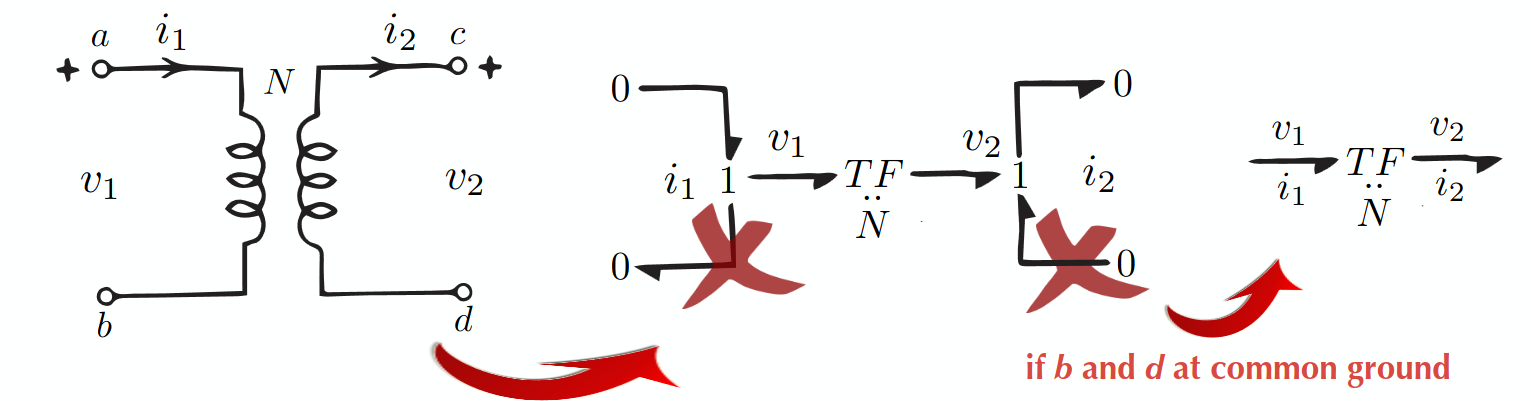
\includegraphics[scale=0.25]{figs/chapter3/3_4.png}
\caption{Ideal transformer with turns ratio $N$.}
\end{figure}


\subsubsection{Electrical Gyrators}

Electrical gyrators are exhibited in Hall effect transducers, where voltage across a semiconductor material is related to a current through the material perpendicular to the voltage drop direction. The same construction method extends to \textbf{electrical networks} containing transformers (TF) and gyrators (GY). The transformer element inserts between two 1-junctions; the turns ratio $N$ becomes the TF modulus. The basic rules for bond graph construction remain unchanged.



\begin{insightbox}[Ladder and T/pi structures]

\begin{figure} [H]
\centering
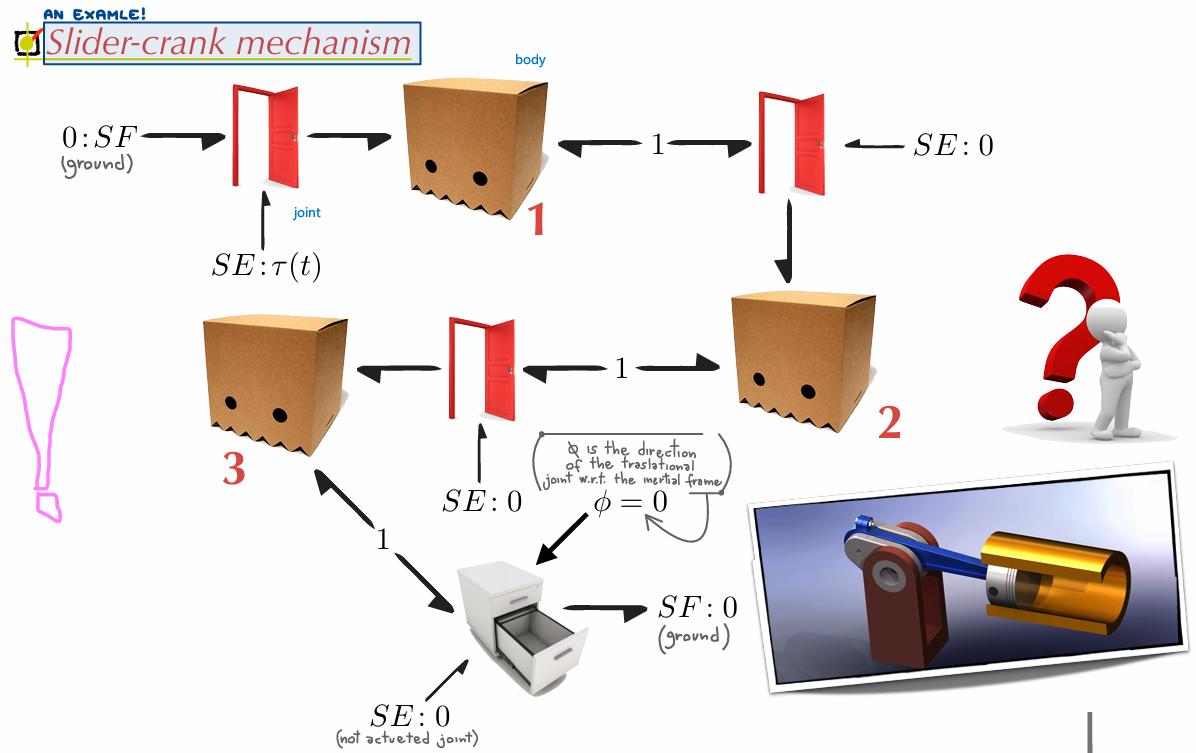
\includegraphics[scale=0.25]{figs/chapter3/3_5.png}
\caption{Resistive ladder with resistors}
\end{figure}

Transmission lines and long hydraulic lines have lumped approximations as ladder networks  cascaded T or pi sections. 
In bond graph terms, the T-section corresponds to alternating 1-junctions (series inductors) and 0-junctions (shunt capacitors). 
The topological dual (exchanging 0 and 1 junctions) gives the pi-section. Notice that the difference between these two schemes is the role of current and voltage is interchanged. This technique holds in general when we want to find the topological dual of even complex circuits: exchange 0 and 1 junctions in the BG!
The pi and tee structures become truncations of the ladder structure that allow for reasonable inclusion of some of the \textbf{transmission line dynamics without having the overall system become too large}. Understanding this duality is a powerful shortcut when building bond graphs by inspection.

\begin{figure} [H]
\centering
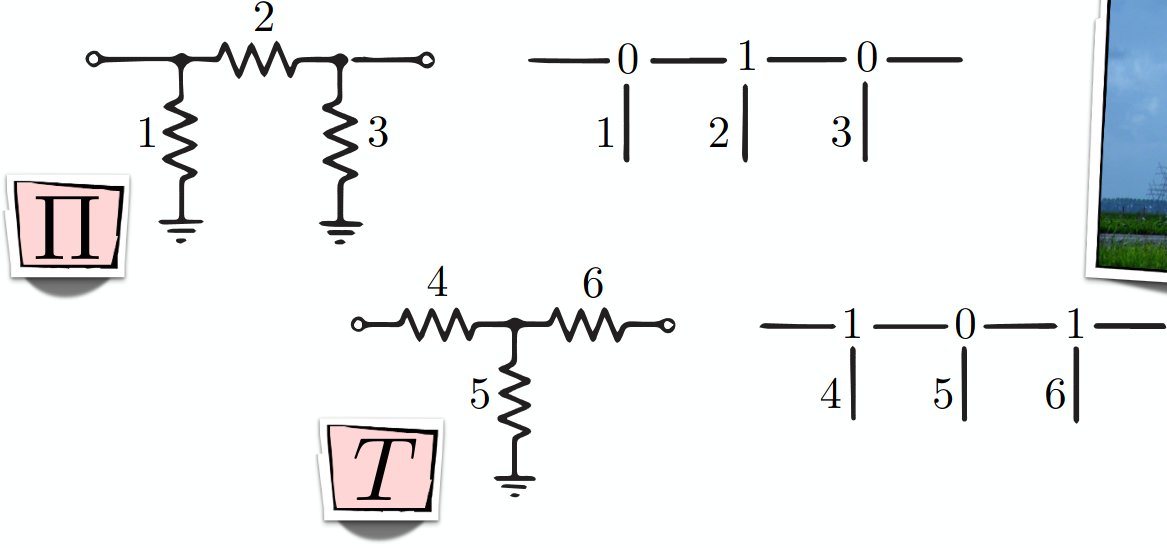
\includegraphics[scale=0.25]{figs/chapter3/3_6.png}
\caption{pi and tee sections as truncations of the ladder structure.}
\end{figure}


\end{insightbox}

\section{Mechanical translation}

Mechanical systems are those composed of components such as masses, springs, dampers, levers, flywheels, gears, shafts, and so forth. When dynamic systems are put together from these components, we must interconnect rotating and translating inertial elements with axial and rotational springs and dampers, and we must appropriately account for the kinematics of the systems.

For mechanical translation, velocity is flow and force is effort. The analogy with electrical circuits is \emph{dual}: in electrical circuits, nodes share voltage (0-junction); in mechanics, rigid connections share velocity (1-junction). 

\begin{itemize}
  \item 0 Junction: Relative velocity (force-generating elements)
  \item 1 Junction: Same velocity
\end{itemize}

\paragraph{Construction procedure for Mechanical Translation.}
\begin{enumerate}[leftmargin=2em,itemsep=2pt]
  \begin{figure} [H]
    \centering
    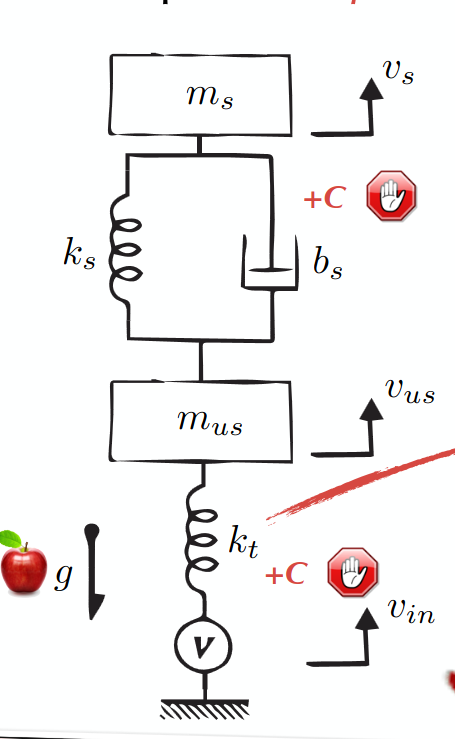
\includegraphics[scale=0.25]{figs/chapter3/3_7.png}
    \caption{Example of mechanical system with translation.}
  \end{figure}

  \item \textbf{Indicate velocity directions}: on a free-body-type sketch, use arrows and symbols to indicate the positive direction of absolute velocity components. Fixing conventional directions in this scheme is the first crucial step! State whether force-generating elements are positive in tension or compression using symbols such as +T or +C.
  \begin{figure} [H]
  \centering
  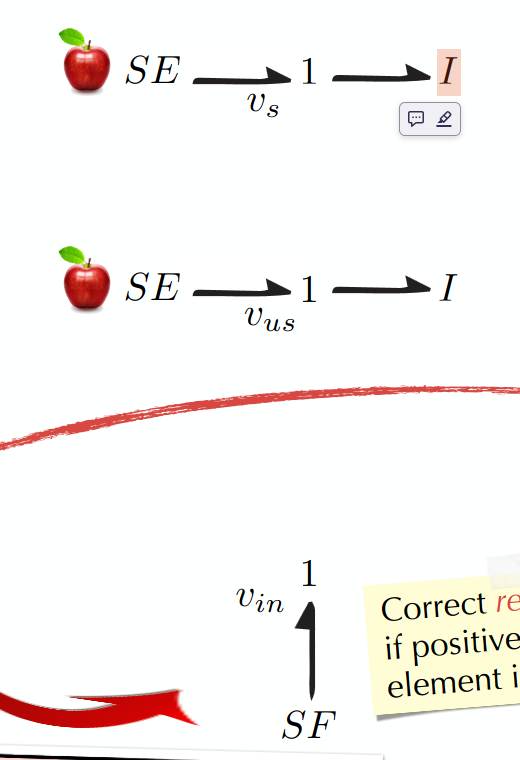
\includegraphics[scale=0.25]{figs/chapter3/3_8.png}
  \caption{Example of free-body sketch with velocity directions and force conventions.}
  \end{figure}

  \item \textbf{One 1-junction per distinct velocity}: each inertia is attached to its absolute velocity 1-junction.
  \item \textbf{0-junctions for relative velocities}: spring and damper forces react to the rate of extension, meaning they depend on the \emph{relative} velocity across them. A 0-junction connecting two 1-junctions produces the relative velocity difference needed by the compliant/resistive element. The sign at the 0-junction must be chosen so that the relative velocity is positive when the element is in the assumed tension/compression state. When forces are positive in tension, power will flow toward the elements.
  

  \begin{figure}[H]
  \centering
  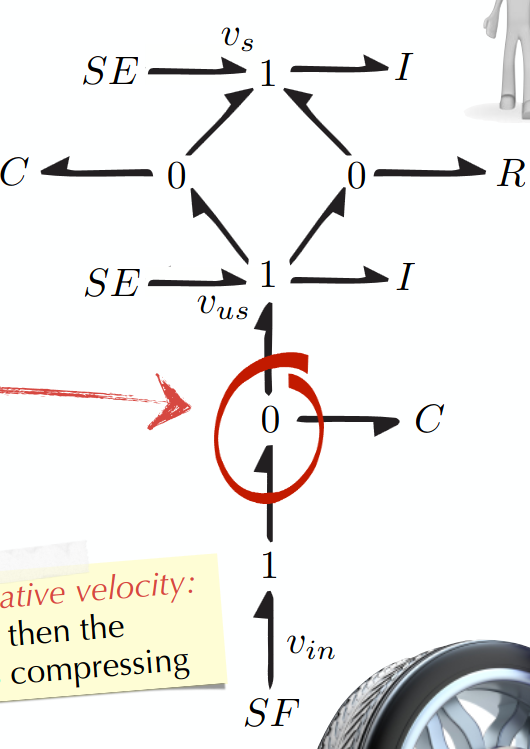
\includegraphics[scale=0.25]{figs/chapter3/3_9.png}
  \caption{Example of bond graph construction for the mechanical system in Fig. 3.7.}
  \end{figure}


  \item \textbf{Reference (ground)}: the inertial frame is fixed in zero velocity, represented by a Sf~: 0, which is deleted after establishing relative velocities.
  \item \textbf{Attach elements}: inertias on 1-junctions; springs (C~: $1/k$) and dampers (R~: $b$) on their relative-velocity 0-junctions; gravity and other absolute forces as Se sources on velocity 1-junctions.
\end{enumerate}

The \emph{beauty} of power conservation in junctions is that we need only to constrain the velocities, and the forces will be automatically balanced without further effort. Newton's second law and the action-reaction principle are built in without explicitly writing them. We can perform a double check to see that the force balance is realized by the 1-junctions.



\paragraph{Reducible loop.}
When a spring and damper are in parallel (same relative velocity), the 0-junction connecting both their velocity 1-junctions can be simplified using bond graph identities into a single 0-junction carrying both the C and R elements. This is the \textbf{reducible loop} , a very common pattern that emphasizes that several elements share exactly the same relative velocity.

\paragraph{Levers, pulleys and kinematic linkages.}
With minor efforts, it is possible to deal with translational systems containing levers, pulleys, and other simple motion-force transforming devices. These introduce position-dependent force/velocity transformations, represented by modulated transformers (MTF) or fixed TF when the geometry is constant. The MTF modulus is the relevant geometric ratio (e.g.\ the Jacobian in robotics).

\section{Fixed-axis rotation}

Fixed-axis rotation occurs in the mechanics of rotating machines, such as electric motors and internal combustion engines, gear boxes, transmissions, transfer cases, differentials, and drive shafts.

Only minor modifications to the procedure for mechanical translation allow handling systems with fixed-axis rotation. It is entirely analogous to translation with the variable substitution $V \to \omega$, $F \to \tau$, $m \to J$, $k \to k_r$, $b \to b_r$. 

The construction procedure is identical: 1-junctions for distinct absolute angular velocities, 0-junctions for relative angular velocity across compliant or resistive rotational elements, TF for gear pairs (modulus = gear ratio $r_1/r_2$), and eliminating the bonds with zero angular velocity.

In the fixed-axis rotation framework, it's not really relevant to talk about +T or +C; what is relevant is to maintain coherence with the relative velocities across all the schemes (e.g., choosing one velocity as the upstream master velocity and the other as the downstream slave velocity).

\begin{figure} [H]
\centering
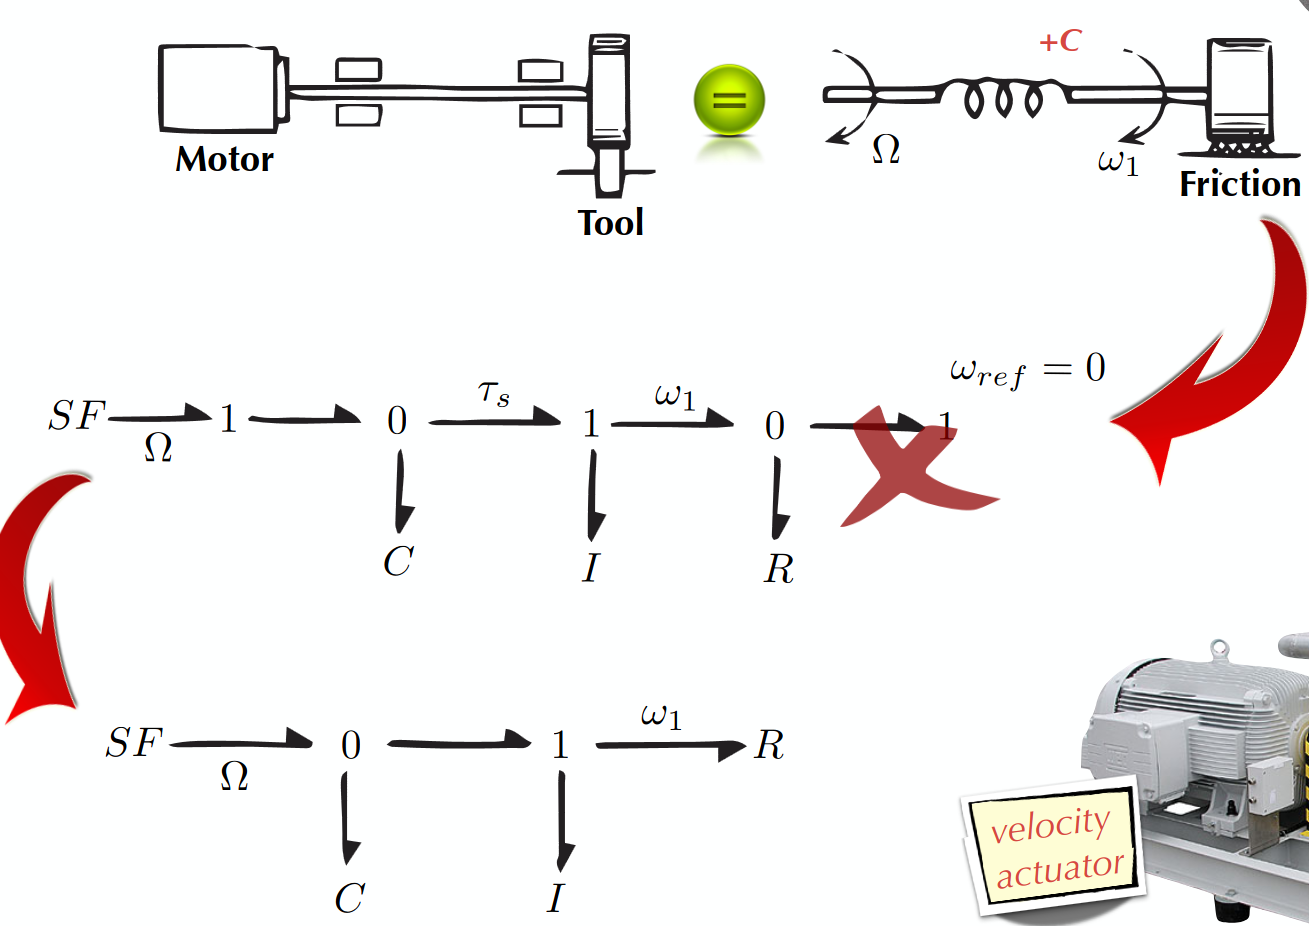
\includegraphics[scale=0.25]{figs/chapter3/3_10.png}
\caption{Example of bond graph construction for a fixed-axis rotational system.}
\end{figure}


\section{Plane motion of rigid bodies}

Mechanical bodies with finite mass both translate and rotate in real applications; their dynamics are governed by a simultaneous combination of translation and rotation. 3-D motion is not trivial, so plane motion is much simpler. Plane motion results when the inertial bodies of a physical system are constrained to translate in two dimensions and to rotate only about an axis perpendicular to the plane of motion. The motion is always w.r.t. an inertial frame (with eventually coordinate transformations in the middle).

When a body both translates and rotates in a plane, three absolute velocity components are needed: $v_x$, $v_y$ (translational velocities of the centre of mass) and $\omega$ (angular velocity). Newton's law in the plane gives three 1-junctions, one per component, each with its own inertia element:

\begin{equation}
  m\dot{v}_x = F_x, \quad m\dot{v}_y = F_y, \quad J\dot{\omega} = \tau,
\end{equation}

\begin{figure} [H]
\centering
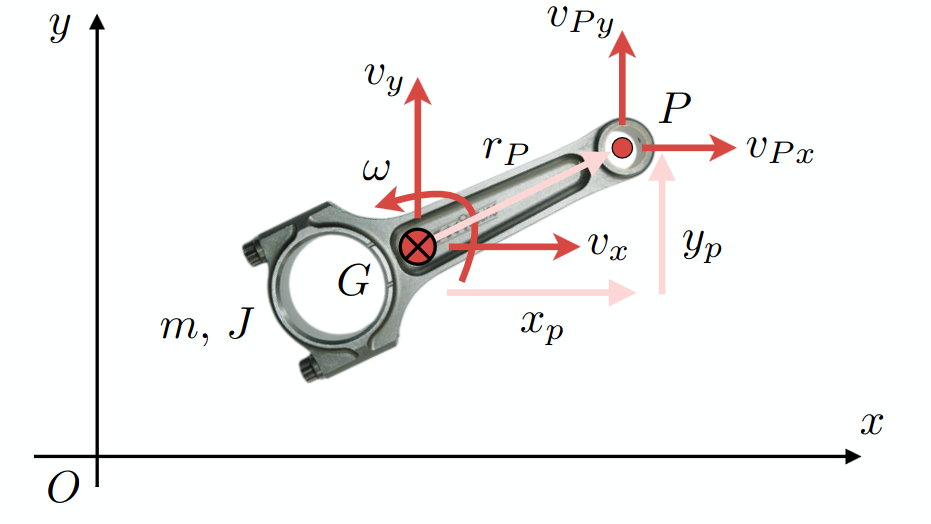
\includegraphics[scale=0.25]{figs/chapter3/3_11.png}
\caption{Mechanical body}
\end{figure}

\begin{figure} [H]
  \centering
  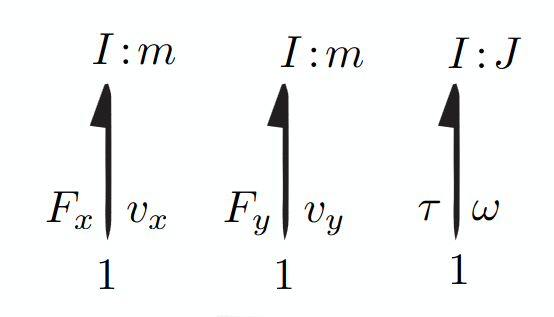
\includegraphics[scale=0.25]{figs/chapter3/3_12.png}
  \caption{Bond graph representation of the plane motion of a rigid body.}

\end{figure}

so the kinetic energy is $T = \frac{1}{2}m v_x^2 + \frac{1}{2}m v_y^2 + \frac{1}{2}J\omega^2$ with three I-elements. This dynamic representation does not involve directly any position information, which is coherent with the fact that this object stores kinetic energy, not potential energy.

Devices are attached at points $P$ offset from the centre of mass by $(r_P\cos\theta, r_P\sin\theta)$ in the inertial frame. The velocity of point $P$ is:
\begin{equation}
  v_{Px} = v_x - (r_P\sin\theta)\omega, \qquad
  v_{Py} = v_y + (r_P\cos\theta)\omega.
\end{equation}
These are linear combinations of the three body-velocity components, implemented with MTF elements (moduli $r_P\sin\theta$ and $r_P\cos\theta$, time-varying through $\theta$). By power conservation ($\Delta F_x v_x + F_y v_y + \tau \omega = F_{Px}v_{Px} + F_{Py}v_{Py} + \tau_P \omega_P$), the corresponding forces and torques at the body's ports are automatically balanced without writing free-body equations explicitly. The result is an "object" with a force/velocity interface toward the environment (what is outside the system). All the port variables are expressed with respect to the inertial frame. 


\begin{insightbox}[Parenthesis: the Body Frame!]
To characterize the energy of a rigid body, it is necessary to know the velocity of the center of mass and the angular velocity. The velocities discussed so far are expressed in the inertial reference, but for multi-body dynamics, it is sometimes convenient to introduce body-fixed coordinates. This coordinate frame remains attached to the center of mass and moves with the body. The advantage is that the inertial tensor is constant, unlike in the inertial frame where it varies with the configuration of the mechanism. 
However, expressing absolute accelerations in the body frame requires additional terms (e.g., $a_x = \dot{v}_X - \omega v_Y$). While body frames are generally preferred to have a constant inertial tensor, in the planar case, inertial frames can be used without any problems.

We can see the body dynamics as a "black box" with three ports (two for translation and one for rotation) that can be connected to the environment. The internal structure of the body is not relevant for the external behavior, which is fully characterized by the kinetic energy and the force/velocity relations at the ports. This is a powerful abstraction that allows us to model complex systems without needing to know all the internal details of each component.

\begin{figure} [H]
  \centering
  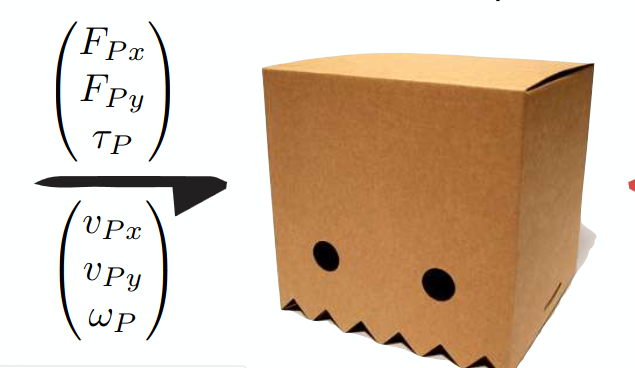
\includegraphics[scale=0.25]{figs/chapter3/3_13.png}
  \caption{Black-box representation of a rigid body with three ports.}
\end{figure}

\end{insightbox}

\paragraph{Connecting rigid bodies: joints.}
Going back to the formulation in the inertial frame, to interconnect rigid bodies and obtain complex mechanisms, it is necessary to define joints that constrain motion in specific directions.
A \textbf{rotational joint} constrains the two connected bodies to have the same position (zero relative linear velocity) while leaving angular velocity free. Any difference in angular velocity ($\omega_r = \omega_B - \omega_A$) means a torque exists.

\begin{figure} [H]
\centering
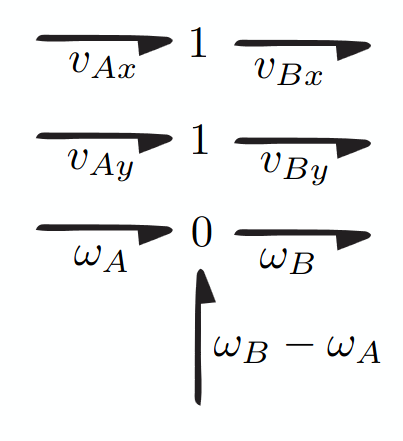
\includegraphics[scale=0.25]{figs/chapter3/3_14.png}
\caption{Rotational joint connecting two bodies.}
\end{figure}


A \textbf{translational joint} constrains relative motion to one direction. Since velocities are in the inertial frame, this direction is not fixed and is related to an angle $\phi$. The relative velocities must be transformed into the direction of the joint.
Both are represented by setting appropriate velocity-difference bonds to zero and using MTF elements for the direction transformation in the inertial frame. This is the basis for the bond graph modelling of robot manipulators and mechanisms.


\begin{figure} [H]
\centering
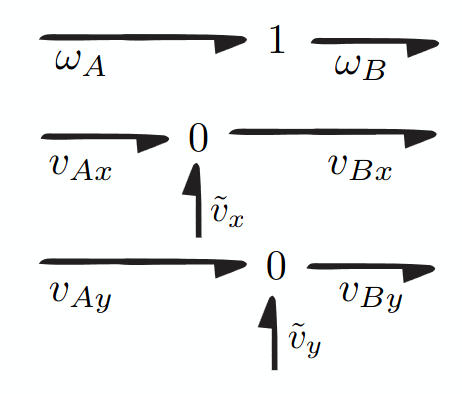
\includegraphics[scale=0.25]{figs/chapter3/3_15.png}
\caption{Translational joint connecting two bodies.}
\end{figure}

\begin{figure}[H]
\centering
% \includegraphics[scale=0.25]{figs/chapter3/3_16.png}
\caption{Rotation of the relative velocity. Instead of dividing by $cos$ and $sin$, we use a trick with a MTF}
\end{figure}


\section{Hydraulic and acoustic circuits}

\begin{itemize}
  \item One category is \textbf{hydrostatic systems}. Typical examples are pumps, motors, pipes, pistons, valves, filters, and accumulators that use nearly incompressible fluids. These systems have high pressures and low fluid velocities so that the \textbf{static pressure dominates the dynamic pressure}. Pressure $P$ is effort, volume flow rate $Q$ is flow.
  \item A second category involves compressible gases where the pressure deviations are small enough that the \textbf{acoustic approximation} applies. In this regime, the gas behaves linearly, sound waves can be described using simplified wave equations, and we can avoid considering thermodynamic effects. Pneumatic systems with large pressure variations need a more complicated modeling treatment.
\end{itemize}

Acoustic approximation refers to a simplified model used for compressible gases, like air, when pressure variations are very small compared to the ambient pressure. In this regime, the gas behaves linearly, and sound waves can be described using simplified wave equations.

\begin{equation*}
  \frac{\partial ^2 p}{\partial t^2} = c^2 \nabla^2 p
\end{equation*}

Where $p$ is the acoustic pressure, and $c$ is the speed of sound in the medium.


\subsection{Fluid Resistance}
A 1-port fluid resistor relates a \textbf{pressure drop} $P_3 = P_1 - P_2$ to a volume flow rate. \textbf{The value of the resistance can be measured experimentally.}

\begin{figure}[H]
  \centering
  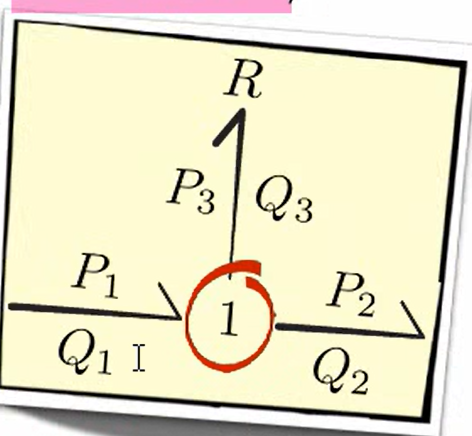
\includegraphics[scale=0.25]{figs/chapter3/3_17.png}
  \caption{Fluid resistor connecting two fluid nodes.}
\end{figure}

\begin{equation*}
  \begin{matrix}
    Q_1 = Q_2 = Q_3 \\
    P_3 = P_1 - P_2 = \Phi_R(Q_3)  = R_3 Q_3 \quad \text{(linear)} 
  \end{matrix}
\end{equation*}

The Reynold number determines if the flow is laminar or turbulent and thus the relationship between pressure drop and flow rate

\begin{equation*}
  Re = \frac{4 \rho Q}{\pi d \mu}
\end{equation*}

\begin{itemize}
  \item If the Reynolds number is low ($Re < 2000$), $P = R Q$, where $R$ is the linear resistance coefficient. This is the regime of laminar flow, where the fluid flows in parallel layers without turbulence.
  \begin{equation*}
    R = 128 \mu l / (\pi d^4)
  \end{equation*}

  \item If the Reynolds number is high ($Re > 5000$), the flow is turbulent, and the pressure drop is given by $P = a_t Q |Q|^{3/4}$, where $a_t$ is a turbulent resistance coefficient.
  
  \item For $2000 < Re < 5000$, the flow is in a transitional regime, and the relationship between pressure drop and flow rate is more complex, often requiring empirical data or more sophisticated models to accurately describe the behavior.

\end{itemize}

\subsubsection{Orifices}
Short obstructions like orifices and valves are important cases where a pressure drop occurs over short lengths. For an orifice with a fixed area, the pressure drop is proportional to the square of the volume flow rate 

\begin{equation*}
  \Delta P = \frac{\rho Q|Q|}{2 C_d^2 A_0^2}
\end{equation*}

where the discharge coefficient $C_d$ depends on the geometry and nonidealities.

\subsubsection{Valves}
For valves, the area $A(x)$ depends on a position coordinate. The position of a mechanical part influences the hydraulic resistance, acting as a transducer linking the mechanical and hydrostatic domains. They can be modeled by variable-resistance elements modulated by a displacement $\dot{x}$.

\begin{equation*}
  \Delta P = \frac{\rho Q|Q|}{ 2 C_d^2(x) A_0^2(x)}
\end{equation*}

It's important to note that elecetrovalevs modeling is a challenging task.

\subsection{Fluid Capacitance}
A fluid capacitor imposes a relationship between a \textbf{pressure and the integral of the volume flow rate}. Essentially is the  volume of fluid.

\begin{figure}[H]
  \centering
  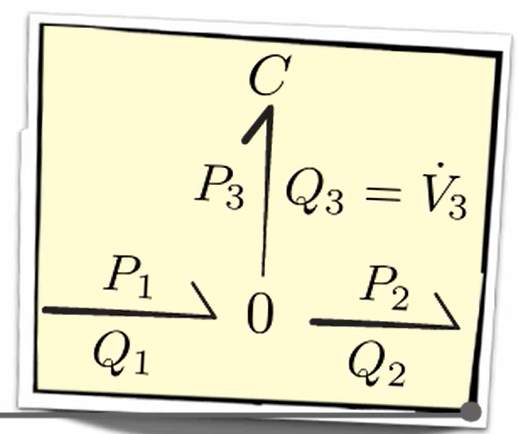
\includegraphics[scale=0.25]{figs/chapter3/3_18.png}
  \caption{Fluid capacitor.}
\end{figure}

\begin{equation*}
  \begin{matrix}
    P_3 = \Phi_C^{-1}(V_3) = \frac{V_3}{C} \\
    V_3 = \int Q_3 dt
  \end{matrix}
\end{equation*}


For a straight-walled water tank in a gravity field,

\begin{equation*}
  P_3 = \rho g h = \rho g \frac{V_3}{A_3}
\end{equation*}
\begin{equation*}
  C_3 = \frac{A_3}{\rho g}
\end{equation*}

\begin{insightbox}[Fluid capacitance as "pressure inertia"]
  The fluid capacitance can be thought as a "Pressure Inertia". Just as a mass resists changes in velocity, a fluid capacitor resists changes in pressure. The larger the capacitance, the more fluid volume is needed to produce a given pressure change, which is analogous to how a larger mass requires more force to achieve the same acceleration.
\end{insightbox}


\subsubsection{Fluid Compressibility}
If and are not equal, represents the rate of compression of the fluid in the pipe. and $V_3$ represents the decrease in volume of the fluid in the segment.

\begin{equation*}
  \begin{matrix}
    dP = - B \frac{dV}{V_0} \\
    \Delta P = \frac{B}{V_0} \Delta V_3 \Longrightarrow C = \frac{V_0}{B}
  \end{matrix}
\end{equation*}

\subsubsection{Elasticity of the vessel}
In the other case, the fluid is incompressible, but the vessel containing it is elastic. The pressure change is related to the change in volume by the bulk modulus of the vessel material. The bulk modulus $B$ is defined as the ratio of the infinitesimal pressure increase to the resulting relative decrease in volume:

The bulk modulus is expressed as:
\begin{equation*}
  B = -V_0 \frac{dP}{dV}
\end{equation*}

\begin{figure}
  \centering
  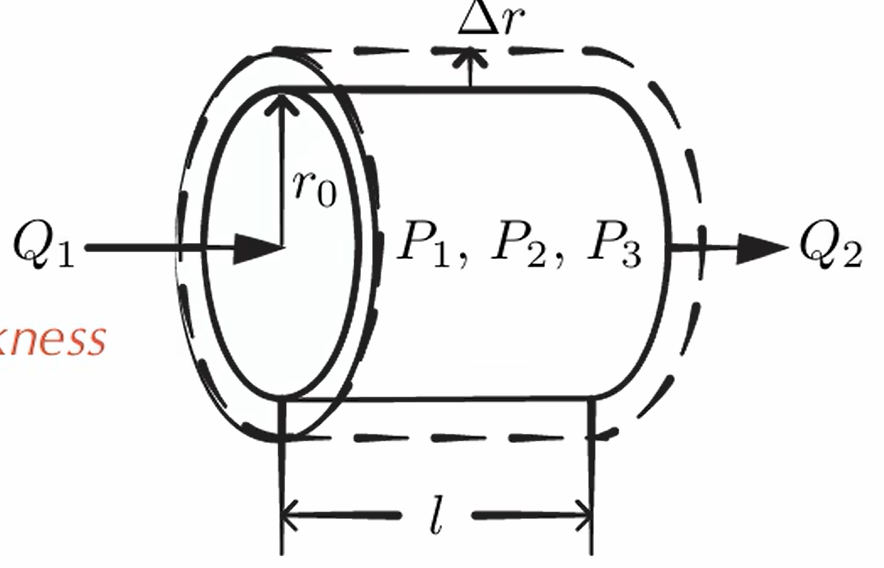
\includegraphics[scale=0.25]{figs/chapter3/3_19.png}
  \caption{Fluid capacitance due to vessel elasticity.}
\end{figure}

\begin{equation*}
  \begin{matrix}
    \sigma = \frac{r_0 P}{t_w} \longrightarrow \text{hoop stress} \\
    \epsilon = \frac{\sigma}{E} = \frac{r_0 P}{t_w E} = \frac{\Delta r}{r_0} \longrightarrow \text{circumferential strain} \\
  \end{matrix}
\end{equation*}

So the change in volume is:

\begin{equation*}
  \begin{matrix}
    \Delta V = \Delta (\pi r^2 l) = \dots = \frac{2 r_0 V_0}{t_w E} P \\
    P_3 = \frac{t_w E}{2 r_0 V_0} V_3 \Longrightarrow C = \frac{2 r_0 V_0}{t_w E}
  \end{matrix}
\end{equation*}

\begin{insightbox}[Capacitance in parallel]
  For cases in which both effect (fluid compressibility and vessel elasticity) contribute, the total capacitance is the sum of the individual capacitances, as they are in parallel. This is because both effects contribute to the overall change in volume for a given pressure change, and their contributions add together to determine the total capacitance of the system.

  \begin{figure}[H]
    \centering
    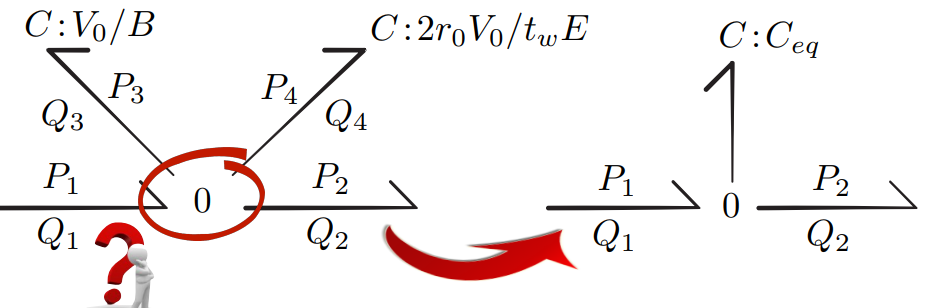
\includegraphics[scale=0.25]{figs/chapter3/3_20.png}
    \caption{Parallel combination of fluid compressibility and vessel elasticity.}
  \end{figure}

  If both fluid compressibility and pipe elasticity contribute, an equivalent compliance can be constructed: $C_{eq} = V_0(\frac{1}{B} + \frac{2r_0}{t_w E})$.

\end{insightbox}


When fluid compliance cannot be modeled with linear behavior, nonlinear models are essential. An example is a gas accumulator with a rubber bladder containing compressed gas. Using the isentropic pressure-volume law 

\begin{figure}[H]
  \centering
  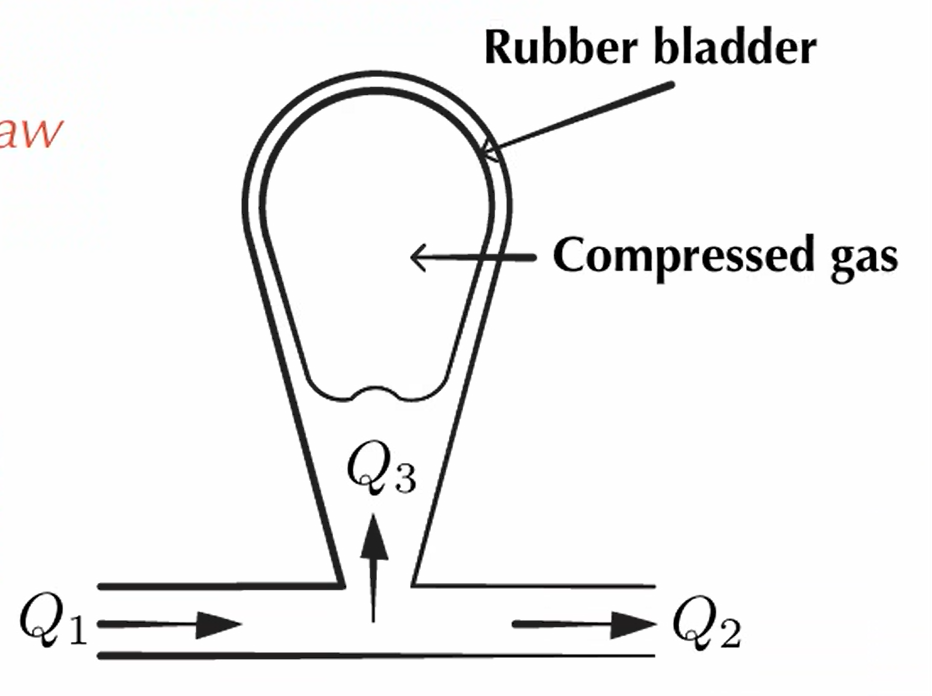
\includegraphics[scale=0.25]{figs/chapter3/3_21.png}
  \caption{Nonlinear fluid capacitor with isentropic behavior.}
\end{figure}

\begin{equation*}
    P V^\gamma = const
\end{equation*}

The pressure is a nonlinear function of the volume: $P_3 = \frac{P_0 V_0^\gamma}{(V_0 - V)^\gamma}$.

\subsection{Fluid Inertia}
Fluid systems have inertia effects analogous to mechanical systems: fluid elements store kinetic energy. The inertia coefficient is related to the parameters of a pipe segment. 

\begin{equation*}
  p_{P_3} = \int P_3 d\tau = \int (P_1 - P_2) d\tau \leftrightarrow I_3 Q_3 = p_{P_3}
\end{equation*}

From Newton's law, a linear inertia coefficient for a pipe of constant cross-section $A$ and length $l$ is $I = \rho \frac{l}{A}$. For a pipe with a non-constant section, $I = \int_0^l \frac{\rho}{A(s)} ds$.

\begin{figure}[H]
  \centering
  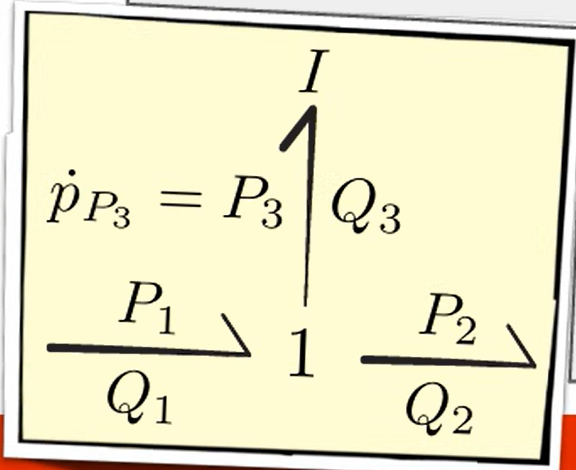
\includegraphics[scale=0.25]{figs/chapter3/3_22.png}
  \caption{Fluid inertia in a pipe segment.}
\end{figure}

\begin{insightbox}[Explaining the fluid inertia]
  The fluid inertia is used to explain the phenomenon that happens when, for instance, a valve is suddenly closed. The fluid in the pipe has kinetic energy (a buildup of momentum), and when the valve is closed, the momentum cannot dissipate immediately, it has to keep flowing until it is dissipated.
\end{insightbox}

\subsubsection{Construction of Hydraulic Bond Graphs}
For both, the construction procedure follows the same 0/1-junction rules as electrical circuits:
\begin{enumerate}
  \item Indicate positive directions for fluid flows and pressures.
  \item For each distinct absolute pressure introduce a 0-junction. Attach elements if they react to one of the absolute pressures. If necessary, include a 0-junction for atmospheric pressure (which can be eliminated if "gauge" pressures are used. Namely, it can be elimnated if all the compoents has a base, the atmospheric pressure).
  \item Insert R-, C-, and I-elements between appropriate 0-junctions using 1-junctions that establish pressure differences acting on the passive elements.
  \item Simplify the graph.
\end{enumerate}

\section{Transducers \& multi-energy domain models}

Transducers are devices that couple subsystems of distinct energy domains. A major reason for studying bond graphs is that they provide a uniform and precise way to represent systems when several forms of power and energy are involved.

\paragraph{Transformer transducers.} 
An ideal transformer transducer, like a hydraulic ram (piston), converts mechanical power to hydraulic power.

\begin{figure}[H]
  \centering
  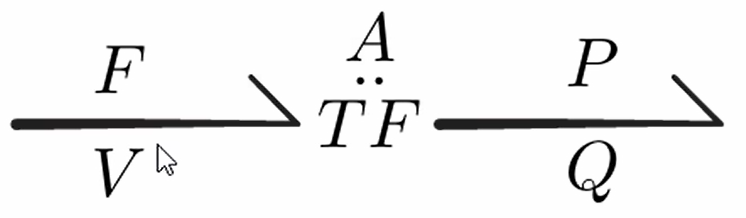
\includegraphics[scale=0.25]{figs/chapter3/3_23.png}
  \caption{Ideal transformer transducer (piston) connecting mechanical and hydraulic domains.}
\end{figure}

\begin{itemize}
  \item Transformer is for the fact that the relation between the two domains is a linear scaling of effort and flow variables. 
  \item Transducer is for the fact that it converts power from one domain to another.
\end{itemize}

\begin{figure}[H]
  \centering
  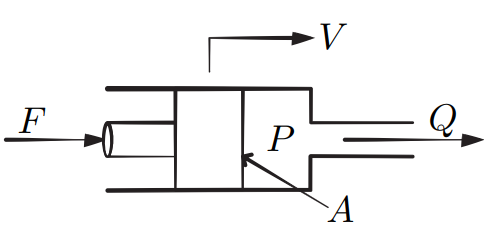
\includegraphics[scale=0.25]{figs/chapter3/3_24.png}
  \caption{Ideal transformer transducer (piston) with idealized power flow.}
\end{figure}

\begin{equation*}
  \begin{matrix}
    F = A P \\
    V = \frac{Q}{A}
  \end{matrix}
\end{equation*}
This applies only to the ideal effects at the face of the piston. Real devices exhibit power losses and energy-storing mechanisms. The process consists of enriching the idealized model. On the mechanical side, we add a 1-junction with a resistor to include friction (which may be dry friction, $F_f = F_0 sgn(V)$, or linear, $F_f = bV$) and an I-element for the piston's mass. On the hydraulic side, a 0-junction and resistance represent leakage, and a C-element models fluid compliance (which may be nonlinear and depend on the nominal extension $x_0$). This complexity can lead to oscillatory phenomena that are damped by the resistance.

\begin{figure}[H]
  \centering
  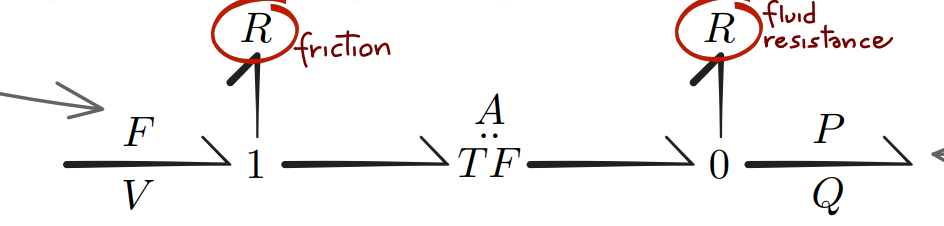
\includegraphics[scale=0.25]{figs/chapter3/3_25.png}
  \caption{Enriched transformer transducer model with losses and energy storage.}
\end{figure}

Positive displacement hydraulic pumps and motors consist of pistons moved by a shaft. With many pistons, the angular speed is related to the flow rate by a nearly constant coefficient: 
\begin{equation*}
  \begin{matrix}
    P_B - P_A = T \tau \\
    T Q = \omega
  \end{matrix}
\end{equation*}

\begin{figure}[H]
  \centering
  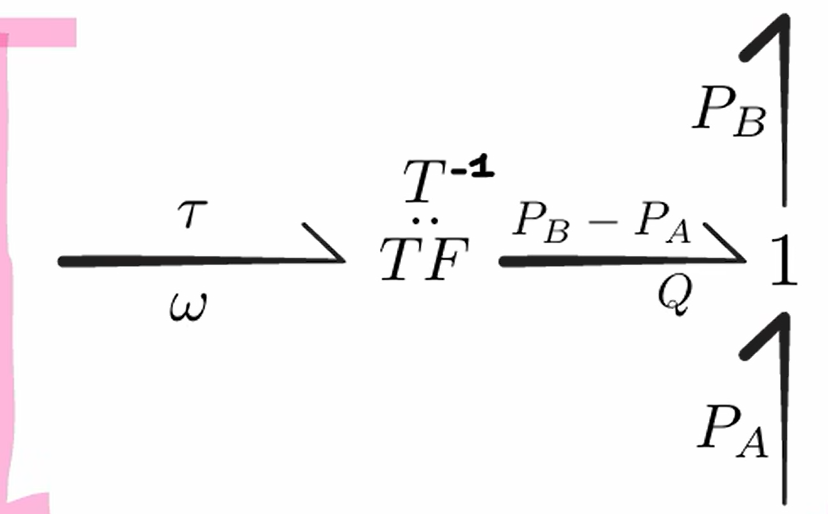
\includegraphics[scale=0.25]{figs/chapter3/3_26.png}
  \caption{Positive displacement hydraulic pump/motor model.}
\end{figure}

  \begin{insightbox}{Enriching the ideal transformer model}
  The ideal transformer model captures the fundamental power conversion mechanism, but it does not account for real-world complexities such as friction, inertia, leakage, and compliance. By enriching the model with additional elements (resistors for losses, I-elements for inertia, C-elements for compliance), we can capture a more accurate representation of the system's behavior. The augmented model can exhibit also non linear phenomena.
  \begin{figure}[H]
    \centering
    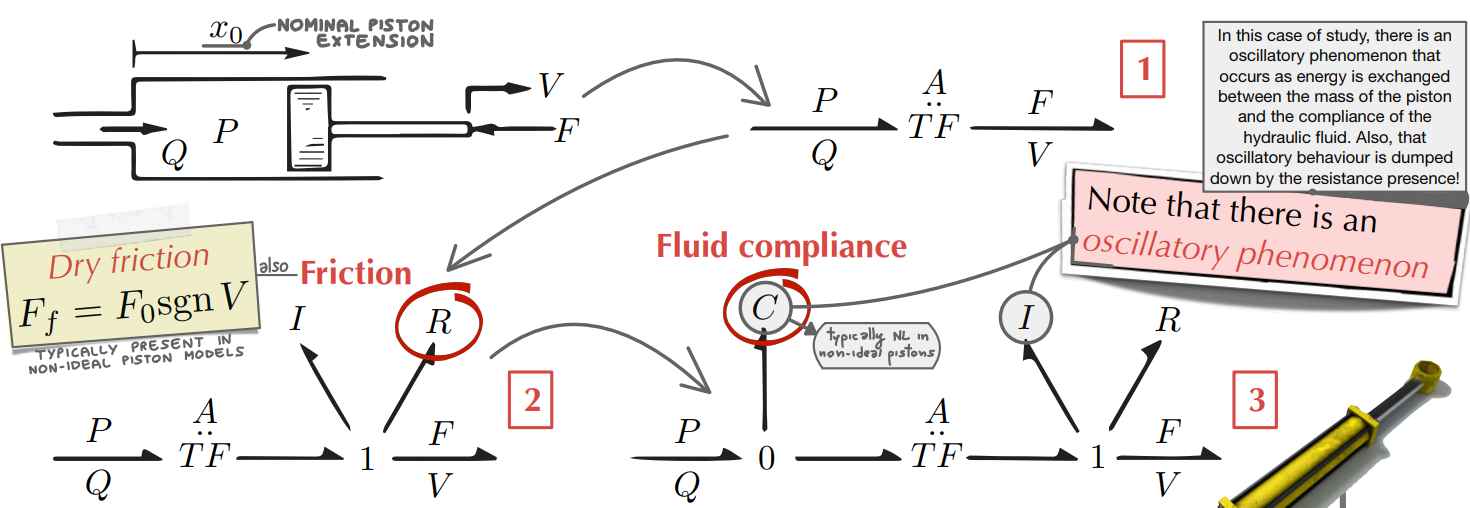
\includegraphics[scale=0.25]{figs/chapter3/3_27.png}
    \caption{Enriched transformer model with additional phenomena.}
  \end{figure}
\end{insightbox}

\paragraph{Gyrator transducers.}
Electromechanical transducers, such as rotary/linear motors or voice coils, use gyrators. A current-carrying conductor moving in a magnetic field experiences an induced voltage (Faraday's law, $e = BlV$) and produces a force (Lorentz force, $Bli = F$). The cross-coupling of effort to flow and flow to effort makes this a gyrator ($e/V = GY = F/i$).

For a DC motor/generator with a commutator, the induced voltage is proportional to the angular speed, and the torque is proportional to the current:

\begin{equation*}
  \begin{matrix}
    e = T \omega \\
    T i = \tau
  \end{matrix}
\end{equation*}

\begin{figure}[H]
  \centering
  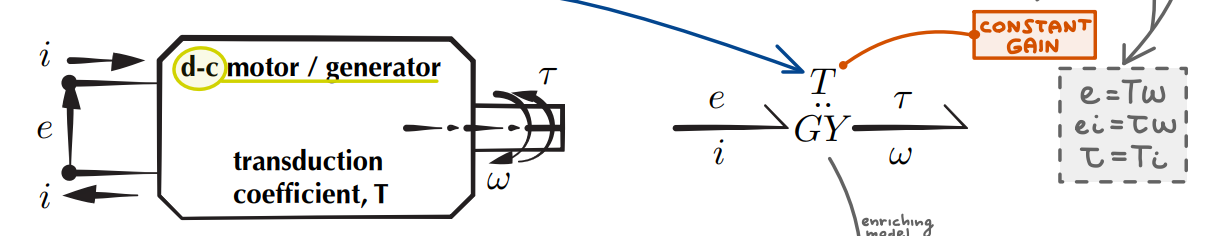
\includegraphics[scale=0.25]{figs/chapter3/3_28.png}
  \caption{Gyrator transducer model for an electromechanical device.}
\end{figure}

A detailed model is developed by adding the winding resistance and inductance, and the rotor's inertia and friction to the basic GY element.

\begin{figure}[H]
  \centering
  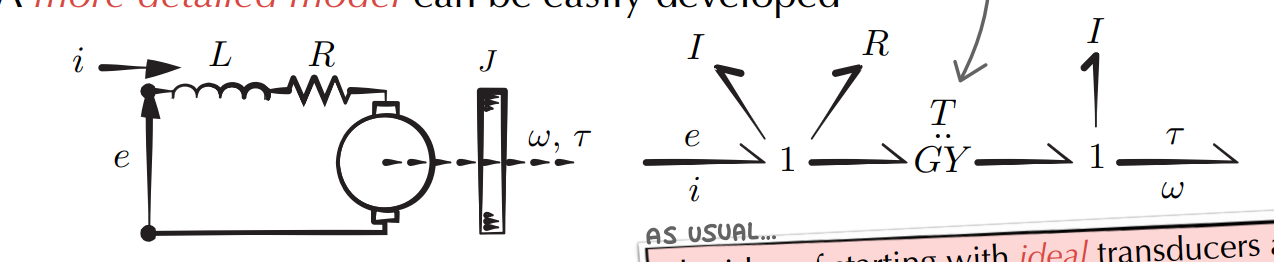
\includegraphics[scale=0.25]{figs/chapter3/3_29.png}
  \caption{Enriched gyrator model with additional phenomena.}
\end{figure}



\paragraph{Modulated Transducers.}
If the gain is time-dependent, MTF and MGY can model more complex power transducers. 

\begin{equation*}
  \left\{\begin{matrix}
    \lambda = n B l_2 l_1 \sin\theta \\
    e = (n B l_2 l_1 \cos\theta) \omega \\
    (n B l_2 l_1 \cos\theta) i = \tau
  \end{matrix}\right.
\end{equation*}

\begin{figure}[H]
  \centering
  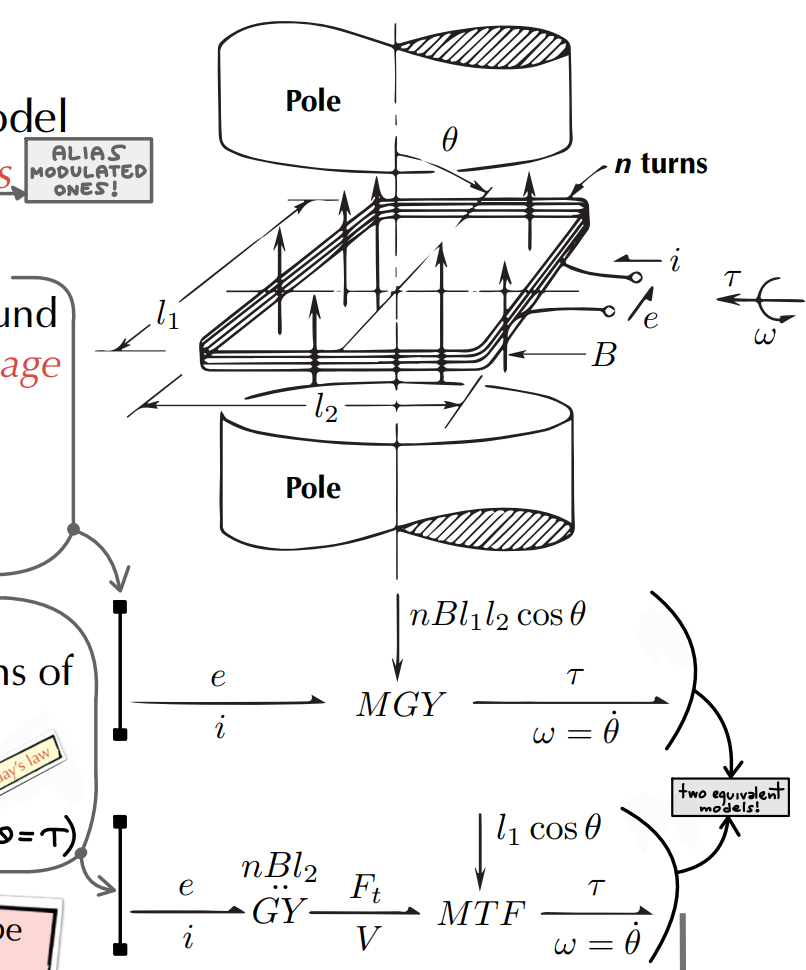
\includegraphics[scale=0.25]{figs/chapter3/3_30.png}
  \caption{Modulated transformer and gyrator transducers.}
\end{figure}